%% bare_jrnl.tex
%% V1.4b
%% 2015/08/26
%% by Michael Shell
%% see http://www.michaelshell.org/
%% for current contact information.
%%
%% This is a skeleton file demonstrating the use of IEEEtran.cls
%% (requires IEEEtran.cls version 1.8b or later) with an IEEE
%% journal paper.
%%
%% Support sites:
%% http://www.michaelshell.org/tex/ieeetran/
%% http://www.ctan.org/pkg/ieeetran
%% and
%% http://www.ieee.org/

%%*************************************************************************
%% Legal Notice:
%% This code is offered as-is without any warranty either expressed or
%% implied; without even the implied warranty of MERCHANTABILITY or
%% FITNESS FOR A PARTICULAR PURPOSE! 
%% User assumes all risk.
%% In no event shall the IEEE or any contributor to this code be liable for
%% any damages or losses, including, but not limited to, incidental,
%% consequential, or any other damages, resulting from the use or misuse
%% of any information contained here.
%%
%% All comments are the opinions of their respective authors and are not
%% necessarily endorsed by the IEEE.
%%
%% This work is distributed under the LaTeX Project Public License (LPPL)
%% ( http://www.latex-project.org/ ) version 1.3, and may be freely used,
%% distributed and modified. A copy of the LPPL, version 1.3, is included
%% in the base LaTeX documentation of all distributions of LaTeX released
%% 2003/12/01 or later.
%% Retain all contribution notices and credits.
%% ** Modified files should be clearly indicated as such, including  **
%% ** renaming them and changing author support contact information. **
%%*************************************************************************


% *** Authors should verify (and, if needed, correct) their LaTeX system  ***
% *** with the testflow diagnostic prior to trusting their LaTeX platform ***
% *** with production work. The IEEE's font choices and paper sizes can   ***
% *** trigger bugs that do not appear when using other class files.       ***                          ***
% The testflow support page is at:
% http://www.michaelshell.org/tex/testflow/



\documentclass[journal]{IEEEtran}
\usepackage[OT1]{fontenc}
%
% If IEEEtran.cls has not been installed into the LaTeX system files,
% manually specify the path to it like:
% \documentclass[journal]{../sty/IEEEtran}





% Some very useful LaTeX packages include:
% (uncomment the ones you want to load)


% *** MISC UTILITY PACKAGES ***
%
%\usepackage{ifpdf}
% Heiko Oberdiek's ifpdf.sty is very useful if you need conditional
% compilation based on whether the output is pdf or dvi.
% usage:
% \ifpdf
%   % pdf code
% \else
%   % dvi code
% \fi
% The latest version of ifpdf.sty can be obtained from:
% http://www.ctan.org/pkg/ifpdf
% Also, note that IEEEtran.cls V1.7 and later provides a builtin
% \ifCLASSINFOpdf conditional that works the same way.
% When switching from latex to pdflatex and vice-versa, the compiler may
% have to be run twice to clear warning/error messages.






% *** CITATION PACKAGES ***
%
%\usepackage{cite}
% cite.sty was written by Donald Arseneau
% V1.6 and later of IEEEtran pre-defines the format of the cite.sty package
% \cite{} output to follow that of the IEEE. Loading the cite package will
% result in citation numbers being automatically sorted and properly
% "compressed/ranged". e.g., [1], [9], [2], [7], [5], [6] without using
% cite.sty will become [1], [2], [5]--[7], [9] using cite.sty. cite.sty's
% \cite will automatically add leading space, if needed. Use cite.sty's
% noadjust option (cite.sty V3.8 and later) if you want to turn this off
% such as if a citation ever needs to be enclosed in parenthesis.
% cite.sty is already installed on most LaTeX systems. Be sure and use
% version 5.0 (2009-03-20) and later if using hyperref.sty.
% The latest version can be obtained at:
% http://www.ctan.org/pkg/cite
% The documentation is contained in the cite.sty file itself.






% *** GRAPHICS RELATED PACKAGES ***
%
\ifCLASSINFOpdf
  % \usepackage[pdftex]{graphicx}
  % declare the path(s) where your graphic files are
  % \graphicspath{{../pdf/}{../jpeg/}}
  % and their extensions so you won't have to specify these with
  % every instance of \includegraphics
  % \DeclareGraphicsExtensions{.pdf,.jpeg,.png}
\else
  % or other class option (dvipsone, dvipdf, if not using dvips). graphicx
  % will default to the driver specified in the system graphics.cfg if no
  % driver is specified.
  % \usepackage[dvips]{graphicx}
  % declare the path(s) where your graphic files are
  % \graphicspath{{../eps/}}
  % and their extensions so you won't have to specify these with
  % every instance of \includegraphics
  % \DeclareGraphicsExtensions{.eps}
\fi
% graphicx was written by David Carlisle and Sebastian Rahtz. It is
% required if you want graphics, photos, etc. graphicx.sty is already
% installed on most LaTeX systems. The latest version and documentation
% can be obtained at: 
% http://www.ctan.org/pkg/graphicx
% Another good source of documentation is "Using Imported Graphics in
% LaTeX2e" by Keith Reckdahl which can be found at:
% http://www.ctan.org/pkg/epslatex
%
% latex, and pdflatex in dvi mode, support graphics in encapsulated
% postscript (.eps) format. pdflatex in pdf mode supports graphics
% in .pdf, .jpeg, .png and .mps (metapost) formats. Users should ensure
% that all non-photo figures use a vector format (.eps, .pdf, .mps) and
% not a bitmapped formats (.jpeg, .png). The IEEE frowns on bitmapped formats
% which can result in "jaggedy"/blurry rendering of lines and letters as
% well as large increases in file sizes.
%
% You can find documentation about the pdfTeX application at:
% http://www.tug.org/applications/pdftex





% *** MATH PACKAGES ***
%
\usepackage{amsmath}
\usepackage{amssymb}
% A popular package from the American Mathematical Society that provides
% many useful and powerful commands for dealing with mathematics.
%
% Note that the amsmath package sets \interdisplaylinepenalty to 10000
% thus preventing page breaks from occurring within multiline equations. Use:
\interdisplaylinepenalty=2500
% after loading amsmath to restore such page breaks as IEEEtran.cls normally
% does. amsmath.sty is already installed on most LaTeX systems. The latest
% version and documentation can be obtained at:
% http://www.ctan.org/pkg/amsmath





% *** SPECIALIZED LIST PACKAGES ***
%
% \usepackage{algorithmic}
% algorithmic.sty was written by Peter Williams and Rogerio Brito.
% This package provides an algorithmic environment fo describing algorithms.
% You can use the algorithmic environment in-text or within a figure
% environment to provide for a floating algorithm. Do NOT use the algorithm
% floating environment provided by algorithm.sty (by the same authors) or
% algorithm2e.sty (by Christophe Fiorio) as the IEEE does not use dedicated
% algorithm float types and packages that provide these will not provide
% correct IEEE style captions. The latest version and documentation of
% algorithmic.sty can be obtained at:
% http://www.ctan.org/pkg/algorithms
% Also of interest may be the (relatively newer and more customizable)
% algorithmicx.sty package by Szasz Janos:
% http://www.ctan.org/pkg/algorithmicx




% *** ALIGNMENT PACKAGES ***
%
%\usepackage{array}
% Frank Mittelbach's and David Carlisle's array.sty patches and improves
% the standard LaTeX2e array and tabular environments to provide better
% appearance and additional user controls. As the default LaTeX2e table
% generation code is lacking to the point of almost being broken with
% respect to the quality of the end results, all users are strongly
% advised to use an enhanced (at the very least that provided by array.sty)
% set of table tools. array.sty is already installed on most systems. The
% latest version and documentation can be obtained at:
% http://www.ctan.org/pkg/array


% IEEEtran contains the IEEEeqnarray family of commands that can be used to
% generate multiline equations as well as matrices, tables, etc., of high
% quality.




% *** SUBFIGURE PACKAGES ***
%\ifCLASSOPTIONcompsoc
%  \usepackage[caption=false,font=normalsize,labelfont=sf,textfont=sf]{subfig}
%\else
%  \usepackage[caption=false,font=footnotesize]{subfig}
%\fi
% subfig.sty, written by Steven Douglas Cochran, is the modern replacement
% for subfigure.sty, the latter of which is no longer maintained and is
% incompatible with some LaTeX packages including fixltx2e. However,
% subfig.sty requires and automatically loads Axel Sommerfeldt's caption.sty
% which will override IEEEtran.cls' handling of captions and this will result
% in non-IEEE style figure/table captions. To prevent this problem, be sure
% and invoke subfig.sty's "caption=false" package option (available since
% subfig.sty version 1.3, 2005/06/28) as this is will preserve IEEEtran.cls
% handling of captions.
% Note that the Computer Society format requires a larger sans serif font
% than the serif footnote size font used in traditional IEEE formatting
% and thus the need to invoke different subfig.sty package options depending
% on whether compsoc mode has been enabled.
%
% The latest version and documentation of subfig.sty can be obtained at:
% http://www.ctan.org/pkg/subfig




% *** FLOAT PACKAGES ***
%
%\usepackage{fixltx2e}
% fixltx2e, the successor to the earlier fix2col.sty, was written by
% Frank Mittelbach and David Carlisle. This package corrects a few problems
% in the LaTeX2e kernel, the most notable of which is that in current
% LaTeX2e releases, the ordering of single and double column floats is not
% guaranteed to be preserved. Thus, an unpatched LaTeX2e can allow a
% single column figure to be placed prior to an earlier double column
% figure.
% Be aware that LaTeX2e kernels dated 2015 and later have fixltx2e.sty's
% corrections already built into the system in which case a warning will
% be issued if an attempt is made to load fixltx2e.sty as it is no longer
% needed.
% The latest version and documentation can be found at:
% http://www.ctan.org/pkg/fixltx2e


%\usepackage{stfloats}
% stfloats.sty was written by Sigitas Tolusis. This package gives LaTeX2e
% the ability to do double column floats at the bottom of the page as well
% as the top. (e.g., "\begin{figure*}[!b]" is not normally possible in
% LaTeX2e). It also provides a command:
%\fnbelowfloat
% to enable the placement of footnotes below bottom floats (the standard
% LaTeX2e kernel puts them above bottom floats). This is an invasive package
% which rewrites many portions of the LaTeX2e float routines. It may not work
% with other packages that modify the LaTeX2e float routines. The latest
% version and documentation can be obtained at:
% http://www.ctan.org/pkg/stfloats
% Do not use the stfloats baselinefloat ability as the IEEE does not allow
% \baselineskip to stretch. Authors submitting work to the IEEE should note
% that the IEEE rarely uses double column equations and that authors should try
% to avoid such use. Do not be tempted to use the cuted.sty or midfloat.sty
% packages (also by Sigitas Tolusis) as the IEEE does not format its papers in
% such ways.
% Do not attempt to use stfloats with fixltx2e as they are incompatible.
% Instead, use Morten Hogholm'a dblfloatfix which combines the features
% of both fixltx2e and stfloats:
%
% \usepackage{dblfloatfix}
% The latest version can be found at:
% http://www.ctan.org/pkg/dblfloatfix




%\ifCLASSOPTIONcaptionsoff
%  \usepackage[nomarkers]{endfloat}
% \let\MYoriglatexcaption\caption
% \renewcommand{\caption}[2][\relax]{\MYoriglatexcaption[#2]{#2}}
%\fi
% endfloat.sty was written by James Darrell McCauley, Jeff Goldberg and 
% Axel Sommerfeldt. This package may be useful when used in conjunction with 
% IEEEtran.cls'  captionsoff option. Some IEEE journals/societies require that
% submissions have lists of figures/tables at the end of the paper and that
% figures/tables without any captions are placed on a page by themselves at
% the end of the document. If needed, the draftcls IEEEtran class option or
% \CLASSINPUTbaselinestretch interface can be used to increase the line
% spacing as well. Be sure and use the nomarkers option of endfloat to
% prevent endfloat from "marking" where the figures would have been placed
% in the text. The two hack lines of code above are a slight modification of
% that suggested by in the endfloat docs (section 8.4.1) to ensure that
% the full captions always appear in the list of figures/tables - even if
% the user used the short optional argument of \caption[]{}.
% IEEE papers do not typically make use of \caption[]'s optional argument,
% so this should not be an issue. A similar trick can be used to disable
% captions of packages such as subfig.sty that lack options to turn off
% the subcaptions:
% For subfig.sty:
% \let\MYorigsubfloat\subfloat
% \renewcommand{\subfloat}[2][\relax]{\MYorigsubfloat[]{#2}}
% However, the above trick will not work if both optional arguments of
% the \subfloat command are used. Furthermore, there needs to be a
% description of each subfigure *somewhere* and endfloat does not add
% subfigure captions to its list of figures. Thus, the best approach is to
% avoid the use of subfigure captions (many IEEE journals avoid them anyway)
% and instead reference/explain all the subfigures within the main caption.
% The latest version of endfloat.sty and its documentation can obtained at:
% http://www.ctan.org/pkg/endfloat
%
% The IEEEtran \ifCLASSOPTIONcaptionsoff conditional can also be used
% later in the document, say, to conditionally put the References on a 
% page by themselves.




% *** PDF, URL AND HYPERLINK PACKAGES ***
%
%\usepackage{url}
% url.sty was written by Donald Arseneau. It provides better support for
% handling and breaking URLs. url.sty is already installed on most LaTeX
% systems. The latest version and documentation can be obtained at:
% http://www.ctan.org/pkg/url
% Basically, \url{my_url_here}.




% *** Do not adjust lengths that control margins, column widths, etc. ***
% *** Do not use packages that alter fonts (such as pslatex).         ***
% There should be no need to do such things with IEEEtran.cls V1.6 and later.
% (Unless specifically asked to do so by the journal or conference you plan
% to submit to, of course. )


% correct bad hyphenation here
\hyphenation{op-tical net-works semi-conduc-tor}
\usepackage{graphicx}
\usepackage{subfigure}
\usepackage{color}
%\usepackage[ruled, vlined]{algorithm2e}
\usepackage{algorithm}
\usepackage{algorithmic}
\renewcommand{\algorithmicrequire}{\textbf{Input:}}
\renewcommand{\algorithmicensure}{\textbf{Output:}}
\usepackage{bm}
\usepackage{booktabs}
\newcommand{\tabincell}[2]{\begin{tabular}[t]{@{}#1@{}}#2\end{tabular}}

\newtheorem{definition}{Definition}

\begin{document}
%
% paper title
% Titles are generally capitalized except for words such as a, an, and, as,
% at, but, by, for, in, nor, of, on, or, the, to and up, which are usually
% not capitalized unless they are the first or last word of the title.
% Linebreaks \\ can be used within to get better formatting as desired.
% Do not put math or special symbols in the title.
\title{A Hierarchical Feature Selection Method for Network Anomaly Detection}
%
%
% author names and IEEE memberships
% note positions of commas and nonbreaking spaces ( ~ ) LaTeX will not break
% a structure at a ~ so this keeps an author's name from being broken across
% two lines.
% use \thanks{} to gain access to the first footnote area
% a separate \thanks must be used for each paragraph as LaTeX2e's \thanks
% was not built to handle multiple paragraphs
%

\author{Jiewen Mao, Dong Jiang, Yongquan Hu, Tongquan Wei, Fuke Shen\\School of Computer Science and Technology, East China Normal University}% <-this % stops a space
% \thanks{M. Shell was with the Department
% of Electrical and Computer Engineering, Georgia Institute of Technology, Atlanta,
% GA, 30332 USA e-mail: (see http://www.michaelshell.org/contact.html).}% <-this % stops a space
% \thanks{J. Doe and J. Doe are with Anonymous University.}% <-this % stops a space
% \thanks{Manuscript received April 19, 2005; revised August 26, 2015.}}

% note the % following the last \IEEEmembership and also \thanks - 
% these prevent an unwanted space from occurring between the last author name
% and the end of the author line. i.e., if you had this:
% 
% \author{....lastname \thanks{...} \thanks{...} }
%                     ^------------^------------^----Do not want these spaces!
%
% a space would be appended to the last name and could cause every name on that
% line to be shifted left slightly. This is one of those "LaTeX things". For
% instance, "\textbf{A} \textbf{B}" will typeset as "A B" not "AB". To get
% "AB" then you have to do: "\textbf{A}\textbf{B}"
% \thanks is no different in this regard, so shield the last } of each \thanks
% that ends a line with a % and do not let a space in before the next \thanks.
% Spaces after \IEEEmembership other than the last one are OK (and needed) as
% you are supposed to have spaces between the names. For what it is worth,
% this is a minor point as most people would not even notice if the said evil
% space somehow managed to creep in.



% The paper headers
\markboth{Journal of \LaTeX\ Class Files,~Vol.~14, No.~8, August~2015}%
{Shell \MakeLowercase{\textit{et al.}}: Bare Demo of IEEEtran.cls for IEEE Journals}
% The only time the second header will appear is for the odd numbered pages
% after the title page when using the twoside option.
% 
% *** Note that you probably will NOT want to include the author's ***
% *** name in the headers of peer review papers.                   ***
% You can use \ifCLASSOPTIONpeerreview for conditional compilation here if
% you desire.




% If you want to put a publisher's ID mark on the page you can do it like
% this:
%\IEEEpubid{0000--0000/00\$00.00~\copyright~2015 IEEE}
% Remember, if you use this you must call \IEEEpubidadjcol in the second
% column for its text to clear the IEEEpubid mark.



% use for special paper notices
%\IEEEspecialpapernotice{(Invited Paper)}




% make the title area
\maketitle

%\tableofcontents
% As a general rule, do not put math, special symbols or citations
% in the abstract or keywords.
\begin{abstract}
Abnormal detection of network traffic is still an important means of preventing network attacks. In the anomaly detection process, researchers need to deal with a large number of features in network traffic. In order to determine whether the network traffic is the most essential feature of the attack, in this paper we propose a hierarchical feature selection method. The method selects the essential features of network traffic through feature clustering method based on correlation coefficient and feature ranking method based on information gain, then it classifies network traffic by decision tree classifier. Experiments show that our method reduces the number of features, and shortens training time comparing with full feature set. By comparison with chi-square feature selection method, our method improves the metrics including accuracy, precision, recall and F1-score.
\end{abstract}

% Note that keywords are not normally used for peerreview papers.
\begin{IEEEkeywords}
feature selection, abnormal detection, feature clustering, correlation coefficient, information gain, decistion tree
\end{IEEEkeywords}






% For peer review papers, you can put extra information on the cover
% page as needed:
% \ifCLASSOPTIONpeerreview
% \begin{center} \bfseries EDICS Category: 3-BBND \end{center}
% \fi
%
% For peerreview papers, this IEEEtran command inserts a page break and
% creates the second title. It will be ignored for other modes.
\IEEEpeerreviewmaketitle




% The very first letter is a 2 line initial drop letter followed
% by the rest of the first word in caps.
% 
% form to use if the first word consists of a single letter:
% \IEEEPARstart{A}{demo} file is ....
% 
% form to use if you need the single drop letter followed by
% normal text (unknown if ever used by the IEEE):
% \IEEEPARstart{A}{}demo file is ....
% 
% Some journals put the first two words in caps:
% \IEEEPARstart{T}{his demo} file is ....
% 
% Here we have the typical use of a "T" for an initial drop letter
% and "HIS" in caps to complete the first word.


% needed in second column of first page if using \IEEEpubid
%\IEEEpubidadjcol
\section{Introduction}
\label{sec:introduction}
\IEEEPARstart{W}{hile} the Internet of Things, 5G technology, the improvement of network bandwidth and new network security testing tools bring convenience to people, malicious traffic and network attacks are still serious threats to Internet users and servers. 
On March 2015, GitHub faced a massive DDoS attack. The attack lasted for one week and caused significant damages\cite{github-2015}. On October 2016, Dyn's DNS servers was attacked for two hours, during that time, internet users directed to Dyn servers were unable to reach some of the marquee brands of the internet\cite{dyn-2016}. On May 2017, the WannaCry ransomware attack bursted and over 200,000 compromised computers across 150 countries were influenced by this virus and economic losses from the cyber attack could reach up to 4 billion dollars\cite{wannacry-2017}.

Traditional anomaly detection methods often only use the header information of the network packets. Wang et.al. \cite{Wang2020CS} proposed a dynamic MLP-based attack detection method. The feature selection process of this paper uses backward selection filter method. It deletes the features which make the accuracy of MLP decreasing more than threshold and the remainings are the selected features. However the method in \cite{Wang2020CS} only uses the header information including source IP, TCP flag, source port, destination port, etc..  % TODO: Add refs.
However, diverse types of network anomalies cannot be distinguish effectively only by packet header information. Even in some types of attacks the malicious users may construct and send the packets elaborately to escape the detection from intrusion detection systems(IDS). Once these packets pass the prevension and propagate in the network, the target computer or network device will be compromised.
To solve this problem, this paper takes the statistical information extracted by aggregated flows besides the header information. Different types of anomalies have different statistical patterns. For example, (D)DoS attacks may have larger counts of packets but stable flow duration, while in brute-force attack the packet counts will be smaller but the curve of flow duration fluctuates drasticly. 
% Network anomaly include not only DDoS attacks but also Botnet\cite{Botnet2009}, infiltration, brute force attacks, zero-day attacks, etc.. They have their own characteristics on the pattern of flow traffic, which will be reflected in statistical characteristics that are different from normal traffic.
% However, traditional anomaly detection methods often only use the header information of the network packets. This may be effective in the face of typical network attacks, but if an attacker carefully constructs network packets whose header information is close to the normal mode, the traditional attack detection method may fail. 

Another problem of statistical detection methods are dimensional explosion. A flow may have more than 30 features in the header alone. Considering the statistical characteristics of all packets in flows, number of features in a network data set will grow rapidly. There may be linear relationships or other associations between these features. If we take all features into consideration, on one hand the efficient of learning and modeling algorithms will decrease, on the other hand it is hard to find the intrinsic cause that can determine whether a flow is an attack.

This paper proposes a hierarchical feature selection method, including three steps of data preprocessing, feature clustering and feature ranking. First, we preprocess the network traffic data. This procedure includes removing features that are clearly not available for statistical analysis, filling or dropping missing data, and encoding labels to numerical values. Second, we propose a feature clustering algorithm based on Pearson correlation coefficient to cluster the features with strong correlation and then select the cluster center. The third step will continue the second step, a feature rank algorithm based on information gain and information gain ratio is used to further filter the features. Finally, we use the decision tree (DT) as a classifier and conduct experiments among our proposed method, the features selected by chi-square testing algorithm and the full feature set. We compare them by the training time and training metrics including accuracy, precision, recall and F1-score. 

The contributions of our paper can be summarized as follow:

\begin{enumerate}
    \item This paper proposes a feature clustering method based on Pearson correlation coefficient, which uses correlation coefficients to define distances and aggregates the features with similar distances, and finds the cluster center as the representative feature of the cluster.
    \item This paper proposes a feature ranking algorithm based on information gain, which sorts the features selected before and choose top $k$ features as the final result of selector.
    \item This paper then analyzes the selected feature subset and explains why they can determine whether a flow is normal or attack.
    \item This paper uses decision tree as classifier to compare selected feature subset using proposed method, chi-square selection method, and the complete feature set on the aspect of training time, accuracy, precision, recall and F1-score.
\end{enumerate}

The remaining part of the paper is organized as follows: Section \ref{sec:related} describes related works. Section \ref{sec:problem} describe the formalization of feature selection problem. Section \ref{sec:methods} introduces our hierarchical feature selection method. Section \ref{sec:evaluation} shows the experiment results and then the results is discussed in Section \ref{sec:discussion}. Finally Section \ref{sec:conclusion} concludes this paper and indicates future works.

\section{Related Works}
\label{sec:related}

Different approaches have been proposed to apply to feature selection to improve the performance of feature selection. H. C. Law et al. propose an expectation-maximization (EM) algorithm to estimate the importance of different features and the best number of components for Gaussian-mixture clustering\cite{Law2004}. EM can avoid running EM many times with different numbers of components and different feature subsets, and can achieve better performance than using all the available features for clustering. Yang et al.\cite{Yang2018} present a modified Network Maximal Correlation (NMC) model as a measure to capture correlation relationships between a characteristic variable and a label variable. The results show the method can obtain an optimal subset of features with faster speed, maximum correlation and minimal redundancy through numerical simulation.

In addition, various of new feature selection approaches have been presented in the past years. Wu et al. \cite{Wu2017}propose a new feature selection algorithm based on features unit (FU), which uses entropy of information to obtain features units and sort them to selected the appropriate one. The results in the UCI datasets show that the FU performs better than MIFS-U and mRMR on the whole. Yassine et al.\cite{Yassine2017} propose a new hybrid filter-wrapper algorithm of feature selection based on pairwise feature selection, which benefits from the speed up and the ease of use of filters and the good performance of wrappers. The results indicate that the selected subset of features by the proposed approach has a good classification performance. Yang et al. \cite{Yang2018a} propose a novel unsupervised feature selection method where constructing similarity matrix and performing feature selection are together incorporated into a coherent model. The results show the proposed approach has better performance to solve the objective function and extensive experiments on face images and benchmark datasets. Ke et al. \cite{Ke2018} propose a redundant window-based optimal feature subset discover algorithm for feature selection, which use the growth algorithm to discover the relevant features and use the shrink algorithm to eliminate the redundant ones. The results show that the method has a good performance in terms of accuracy and scalability, and improves the execution efficiency of feature selection and traffic classification.

Liu et al. \cite{Liu2018} propose a differentially private ensemble feature selection algorithm based on output perturbation. The results also demonstrate the high performance under certain privacy preservation degree of the method. Ferriyan et al. \cite{Ferriyan2017} propose a new feature selections using Genetic Algorithm to find the optimal features from NSL-KDD Cup 99 dataset, which use one-point crossover for the Genetic Algorithm parameters instead of two-point crossover. The results show the proposed approach performs better in classification rate and the training time compared to several other classifiers. Han et al. \cite{Han2020} propose a novel unsupervised feature selection method via the graph matrix learning and the low-dimensional space learning to obtain their individually optimized result. The results on real datasets verified that the method achieved the best classification performance compared to the state-of-the-art feature selection methods.

Feature selection also have been broadly used in processing traffic data. Shi et al. \cite{Shi2017} propose a novel feature extraction and selection approach to provide the optimal and robust features for traffic classification, which based on multifractal features, the observation of the multifractal features and the analysis of PCABFS. The results show the approach achieves better classification performance, lower runtime performance and more effective for real-time traffic classification compared to the TLS features. Moreover, the authors then propose a new feature optimization approach based on deep learning and Feature Selection (FS) techniques\cite{Shi2018} to provide the optimal and robust features for traffic data sets. The results show the approach achieves the best classification performance and relatively higher runtime performance compared with the approaches used in the previous work.

Moreover, there are different feature selection methods aim to process different kinds of data. Dong et al.\cite{Dong2017} propose a fine grained classification scheme which based on a hierarchical kNN classifier for network video traffic. The results show that the proposed method outperforms existing methods applying commonly used flow statistical features. Taskin et al. \cite{Taskin2017} presented a novel feature-selection method based on High Dimensional Model Representation (HDMR) to analyze and test in classification of hyperspectral images. The results show that the proposed approach can be used as a fast and efficient feature-selection method yielding very competitive results compared to the state-of-art feature-selection methods. Valadi et al.\cite{Valadi2019} propose a new modification of attribute selection with multiple label which can be advantageously used for handling high dimensional multi-level datasets. The results show the proposed approach reduces complexity and computational run time.

\begin{figure*}[!htbp]
    \centering
    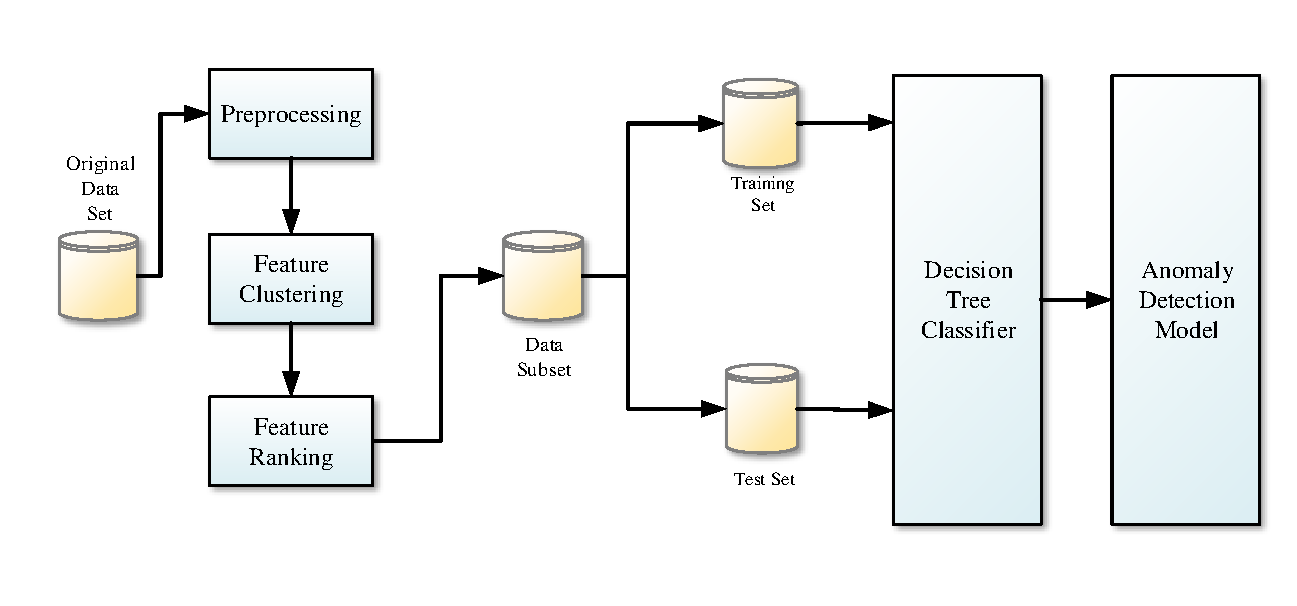
\includegraphics[scale=0.8]{fig/Framework.pdf}
    \caption{Detection Framework}
    \label{fig:framework}
\end{figure*}

\section{Problem Definition and Solution}
\label{sec:problem}
We denote 
$$D=\left(\begin{array}{llll}
    \bm{x}_1 & \bm{x}_2 & \ldots & \bm{x}_m
\end{array}\right)^T$$
as the data set with $m$ instances, where 
$$\bm{x}_i = \left(\begin{array}{lllll}
    f_{1i} & f_{2i} & \ldots & f_{ni} & c_i
\end{array}\right)$$
where $f_{ji}$ is the value of $j$th feautre of vector $\bm{x_i}$, and $f_j \in F = \{f_1, f_2, \ldots, f_n\}$ is the feature set. $c_i$ is the class label of $\bm{x}_i$ and $c_i \in C = \{c_1, c_2, \ldots, c_k\}$, where $C$ is the set of class labels.

The feature selection problem\cite{Maza2018} can be described as a 6-tuple $FS=\langle D, F, C, S, fs, E \rangle$, where $D, F, C$ are data set, feature set and class label set respectively. $S=\{s_1, s_2, \ldots, s_l\}, \ l=2^n-1$ is the search space, which contains all subsets can be constructed from $F$ with $s_i=\{f_j, f_k, \ldots, f_l\}, \ (1 \leqslant j \neq k \neq l \leqslant n)$. $E$ is the evaluation measure and $fs$ represents the function of process of feature selection: $fs: F \rightarrow S$.

The target of the function $fs$, which is the proposed algorithm, is to find the best feature subset $\hat{F} \subset F$. The feature subset should satisfy following conditions:
\begin{itemize}
    \item Every feature $f \in \hat{F}$ is independent with others. It means that every $f$ should not be calculated from other features.
    \item The feature subset $\hat{F}$ is the least set of $s_l$ with given count of features $l$. This feature subset should has enough information to determine whether a flow is an attack or not. If the feature set add or remove any other features, the result of detection will deteriorate.
\end{itemize}

To find such feature subset, we propose our hierarchical feature selection algorithm, which is presented in next Section.

\section{Hierarchical Feature Selection Method}
\label{sec:methods}

\subsection{Overview}

The system framework of this paper is shown as Fig. \ref{fig:framework}. 
The proposed method is the first block in the figure, and it contains three steps or layers: The first step is preprocessing, which cleans data set and makes it to a better form to be processed in next two steps. The second step is feature clustering, which puts all features with potential linear correlation into the same cluster, then all cluster centers are chosen as the representative of every clusters. The third step is feature ranking, which further rank all features selected in step 2 and choose the top $k$ features as the final feature set. 

After the three-steps processing, the refined data subset is divided into training set and test set, then they are trained and tested via decision tree classifier and our detection model is generated.

In following subsections the details and algorithms of proposed methods are described.

\subsection{Data Set and Preprocessing}

The data set being studied is CIC-IDS-2018\cite{cic2018}. 
It is generated on a simulated network topology on the AWS computing platform. The network topology is shown as Figure \ref{fig:topology}. It has 5 subnet and 1 attacker network.  
The data set consists of seven different attack scenarios: Brute-force, Heartbleed, Botnet, DoS, DDoS, Web attacks, and infiltration of the network from inside. It includes the captured network traffic and system logs of each machine, along with 76 features extracted from the captured traffic using CICFlowMeter-V3\cite{cicflowmeter}. These 76 features are shown in Table \ref{tab:features}.

\begin{figure}[!htbp]
    \centering
    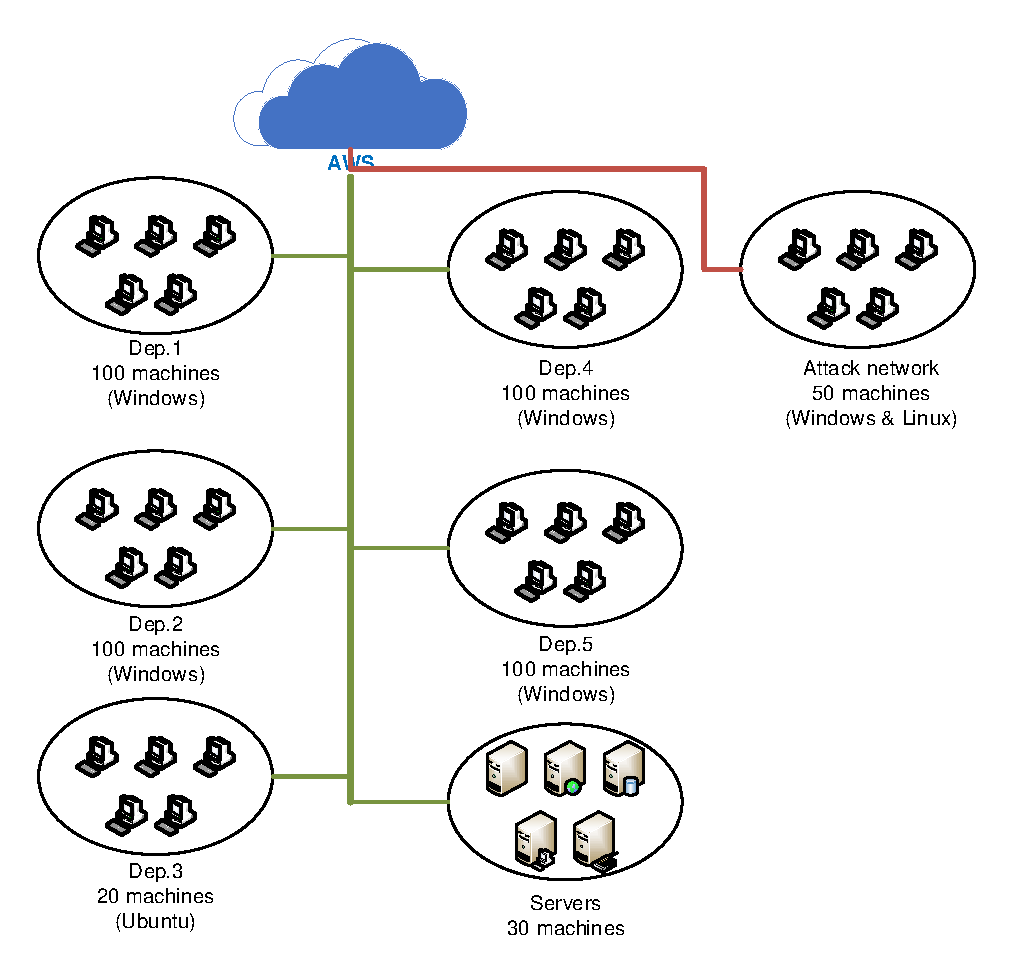
\includegraphics[scale=0.5]{fig/Topology.pdf}
    \caption{Simulated network topology on AWS computing platform}
    \label{fig:topology}
\end{figure}

\begin{table*}[!htpb]
    \caption{76 Features of CIC-IDS-2018 data set}
    \label{tab:features}
    \centering
    \begin{tabular}{llll}
    \toprule
    \multicolumn{4}{c}{Features} \\
    \midrule
    Flow Duration & Total Forward Packets & Total Backward Packets & Total Length Forward Packets \\
    Total Length Backward Packets & Forward Packet Length Max & Forward Packet Length Min & Forward Packet Length Mean \\
    Forward Packet Length Std & Backward Packet Length Max & Backward Packet Length Min & Backward Packet Length Mean \\
    Backward Packet Length Std & Flow Bytes/s & Flow Packets/s & Flow IAT Mean \\
    Flow IAT Std & Flow IAT Max & Flow IAT Min & Forward IAT Total \\
    Forward IAT Mean & Forward IAT Std & Forward IAT Max & Forward IAT Min \\
    Backward IAT Total & Backward IAT Mean & Backward IAT Std & Backward IAT Max \\
    Backward IAT Min & Forward PSH Flags & Backward PSH Flags & Forward URG Flags \\
    Backward URG Flags & Forward Header Length & Backward Header Length & Forward Packets/s \\
    Backward Packets/s & Packet Length Min & Packet Length Max & Packet Length Mean \\
    Packet Length Std &  Packet Length Var & FIN Flag Count & SYN Flag Count \\
    RST Flag Count & PSH Flag Count & ACK Flag Count & URG Flag Count \\
    CWE Flag Count & ECE Flag Count & Down/Up Ratio & Packet Size Avg \\
    Forward Seg Size Avg & Backward Seg Size Avg & Forward Byts/b Avg & Forward Packets/b Avg \\
    Forward Blk Rate Avg & Backward Byts/b Avg & Backward Packets/b Avg & Backward Blk Rate Avg \\
    Subflow Forward Packets & Subflow Forward Byts & Subflow Backward Packets & Subflow Backward Byts \\
    Init Forward Win Byts &  Init Backward Win Byts &   Forward Act Data Packets & Forward Seg Size Min \\
    Active Mean & Active Std & Active Max & Active Min \\
    Idle Mean & Idle Std & Idle Max & Idle Min \\
    \bottomrule
    \end{tabular}

\end{table*}

In order to detect all types of attacks as much as possible, we integrated the network traffic data that was originally scattered in each day, and extracted 20\% of the data as our main data set while maintaining the label ratio. At the same time, in order to ensure the generalization ability of the model, we randomly select and generate data sets as many times as possible. Finally we get 10 stratified-sampled data set files. 

At this moment, the data set is still unavailable because there are some useless nominal features which are not suitable for statistical analyzing, and there may be missing values in the data set. We must remove these features to prevent them interfering proposed algorithms.

Our preprocessing strategy is described as follows:

\subsubsection{Data cleaning}
The target of this paper is to find the decisive statistical features which can determine whether a network flow is an attack. 
So the traditional 5-tuple, i.e. source IP address, source port, destination IP address, destination port and protocol cannot be used to our algorithm. 
These nominal features will be removed to focus on other statistical features. 
We also remove timestamp feature because our algorithm focuses on the type of attacks rather than the time characteristics.

Many missing values also exist in the data set. There are many reasons for missing values. Some flows cannot be calculated in certain features. For example, if the duration time of a flow is too small even equals 0, the values of two features named ``Flow Bytes/s'' and ``Flow Packets/s'' can be NaN or infinity. It is a difficult work to examine every missing value, and they cannot be filled using interpolation because the data set is composed randomly. In this situation, we remove these rows containing missing values to ensure our algorithm running normally.

Note that the removed features are only in the context of this paper. These features may be useful in other detection methods.

\subsubsection{Remove all zero-variance features}

Variance is a physical quantity used to describe the degree of discreteness of a variable. In a data set, if the variance of a feature is zero, it means that this feature has only one value. Thus this feature cannot import any new information to help training the model. We remove these features to refine the data set.

\subsubsection{Encode labels}

Most anomaly detection models perform as classifiers which predict output labels by calculating the probabilities of every label in the label set. The models use input data to train a function. Both input data and output data are often numeric. However in our data set, the labels are text which cannot be processed by detection model. Thus we encoder the labels and map them to numeric values.

\subsection{Layer 1: Feature Clustering Algorithm based on Pearson Correlation Coefficient}

% Many features of the original data set are derived from others. According to our observation, there are linear correlations between many features. The most important step of our method is to merge these linear related features via clustering method. First the concept of correlation coefficient is reviewed.

According to our observation, many features are potentially linear related. For example, in Figure \ref{fig:correlated-variables}, we pick up two pairs of features to show their potential linear correlation. The left part shows that features ``Flow IAT Mean'' and ``Forward IAT Mean'' may have positive correlation. In fact the interval time of a whole flow consists of the forward flow. In the right part, we can see that the feature ``Backward Segment Size Average'' is almost equals to ``Backward Packet Length Mean''. We can treat them as the same feature. 

The redundancy of features is produced by the featrue extraction tool. If we use the whole data set to train our model, the redundant features on one hand may increase the computation and spend more time, on the other hand these redundant features cannot import any new informations into our model. So it is necessary to merge these redundant features. In this paper, we use clustering method to reach this target. 

First the concept of correlation coefficient is reviewed.

\begin{figure}
    \centering
    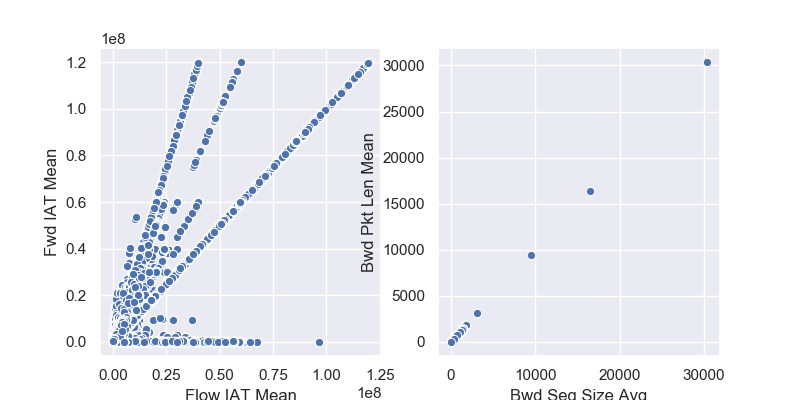
\includegraphics[scale=0.42]{fig/scatter_correlated_variables.png}
    \caption{Two examples of correlated variables. The feature ``Flow IAT Mean'' and ``Forward IAT Mean'', ``Backward Segment Size Average'' and ``Backward Packet Length Mean'' are potentially related. }
    \label{fig:correlated-variables}
\end{figure}

\begin{definition}[Correlation Coefficient]
    If the variances $\sigma^2_X$ and $\sigma_Y^2$ of two random variables $X$ and $Y$ exists and they satisfy that $\sigma^2_X > 0$ and $\sigma^2_Y > 0$, the correlation coefficient of $X$ and $Y$ can be denoted as
\begin{equation}
    \text{Corr}(X, Y) = \frac{\text{Cov}(X, Y)}{\sigma_X \sigma_Y}
\end{equation}
where $\text{Cov}(X, Y)$ is the covariation of $X$ and $Y$. And
$$\text{Corr}(X, Y) \begin{cases}
    > 0, & X \text{ and } Y \text{ are positive correlated.}\\
    = 0, & X \text{ and } Y \text{ are not linear correlated.} \\
    < 0, & X \text{ and } Y \text{ are negative correlated.}
\end{cases}$$
\end{definition}

Then we use the correlation coefficient to define the distance of any two features.

\begin{definition}[The distance of two features]
\label{def:distance}
The distance of two features $f_i$ and $f_j$ is the reciprocal of the absolute value of correlation coefficient of them, that is
\begin{equation}
    \label{eq:distance}
    d(f_i, f_j) = \frac{1}{|\text{Corr}(f_i, f_j)|}
\end{equation}
\end{definition}

According to Equation \ref{eq:distance}, if two features have potential linear correlation, the distance between them is small. On the contrary, if the distance between two features are large, these two features are independent relatively. Here we consider both positive correlation and negative correlation are the same, so we use absolute value of the correlation coefficient. However, the more indepent two features are, the less absolute correlation coefficient of them is. This is the exact opposite of our general definition of distance. Hence we use reciprocal to solve this problem.

The clustering algorithm is described as Algorithm \ref{alg:clustering} and Algorithm \ref{alg:compare-and-join}. We calculate the distance between every feature and others. If the distance is less than a threshold $\delta$, the feature is treated as linear related with the other and they belong to the same cluster. Otherwise, the feature will be put in a new cluster. The procedure ``compare\_and\_join'' at the 4th line of Algorithm \ref{alg:clustering} is complicated, so we list it as Algorithm \ref{alg:compare-and-join}.

\begin{algorithm}
\caption{Feature clustering}
\label{alg:clustering}
\begin{algorithmic}[1]
\REQUIRE ~~\\
    Data set $D=(\bm{x}_1,\bm{x}_2,\ldots,\bm{x}_M)^\text{T}$, \\
    feature set $F=(f_1,f_2,\ldots,f_N)$, \\
    distance threshold $\delta$.
\ENSURE ~~\\
    Cluster set $C=\{c_1,c_2,\ldots,c_K\}$
\STATE $C \gets \emptyset$
\FOR{$i=1,2,\ldots,n$}
    \IF{$\nexists c \in C\ \text{s.t.} f_i \in c$}
        \STATE cluster $c_{join} \gets \text{compare\_and\_join}(D, f_i, C, \delta)$
        \IF{$\exists c_{join}$ which $f_i$ can join}
            \STATE $c_{join}\text{.add}(f_i)$
        \ELSE
            \STATE Create a new cluster $c'$
            \STATE $c'\text{.add}(f_i)$
            \STATE $C\text{.add}(c')$
        \ENDIF
    \ENDIF
\ENDFOR
\RETURN $C$
\end{algorithmic}
\end{algorithm}

\begin{algorithm}
\caption{Compare new feature to all features of all existing cluster}
\label{alg:compare-and-join}
\begin{algorithmic}[1]
\REQUIRE ~~\\
    Data set $D=(\bm{x}_1,\bm{x}_2,\ldots,\bm{x}_M)^\text{T}$, \\
    feature $f_i$, \\
    distance threshold $\delta$,
    currently existing clusters $C=\{c_1, c_2, \ldots, c_K\}$
\ENSURE ~~\\
    A integer $c_{join}$ which indicate the cluster which $f_i$ can join in.  
\STATE A vector including all maximum values of all existing cluster $\bm{d}_{\max}(C) \gets \emptyset$
\FOR{$k=1,2,\ldots,K$}
    \STATE Distance vector for cluster $c_k$, i.e.$\bm{d}(c_k) \gets \emptyset$
    \FOR{$j=1,2,\ldots, \text{sizeof}(c_k)$}
        \STATE $d=1/|\text{Corr}(D^{(f_i)}, D^{(f_j)})|$
        \STATE $\bm{d}(c_k)\text{.add}(d)$
    \ENDFOR
    \STATE $\bm{d}_{\min}(C)\text{.add}(\min{\bm{d}(c_k)})$
\ENDFOR
\STATE Minimum distance in cluster $c_k$ denoted as $d_{\min}=\min{\bm{d}_{\min}(C)}$
\IF{$d_{\min} < \delta$}
    \STATE $c_{join}=\arg\min_c{\bm{d}_{\min}(C)}$
    \RETURN $c_{join}$
\ELSE
    \RETURN NULL
\ENDIF
\end{algorithmic}
\end{algorithm}

After the clusters are generated, next step is to find the center of these clusters. This procedure is listed as Algorithm \ref{alg:find-cluster-center}. We calculate the average distance of every feature between others in each cluster, then we pick the feature with minimum average distance with other features as the center of this cluster. If a cluster only have two features, the algorithm will select the first feature in the cluster as the center of it.

\begin{algorithm}
\caption{Find the cluster center}
\label{alg:find-cluster-center}
\begin{algorithmic}[1]
\REQUIRE ~~\\
    Data set $D=(\bm{x}_1,\bm{x}_2,\ldots,\bm{x}_M)^\text{T}$, \\
    clusters $C=\{c_1, c_2, \ldots, c_K\}$ calculated in Algorithm \ref{alg:clustering}
\ENSURE ~~\\
    A feature list $F'=\{f'_1, f'_2, \ldots, f'_K\}$ whose features are the center of every cluster. 
\STATE Feature list $f'=\emptyset$
\FOR{$i=1,2,\ldots, K$}
    \IF{sizeof($c_i$) = 1}
        \STATE $F'$.add($f \in c_i$)
    \ELSIF{sizeof($c_i$) = 2}
            \STATE select a feature randomly
            \STATE $F'$.add($f \in c_i$)
    \ELSE
        \FOR{each $f \in c_i$}
            \STATE $\bar{d_f}=1/(|c_i|-1)\sum d_{f, f'}$
        \ENDFOR
        \STATE $f_c=\arg\min_f d_c$
        \STATE $F'$.add($f_c$)
    \ENDIF
\ENDFOR
\RETURN $F'$
\end{algorithmic}
\end{algorithm}

\subsection{Layer 2: Feature Ranking Algorithm based on Information Gain}

After the procedure of Layer 1, we generate a group of features which are pairwise independent. In order to further refine the feature space of our data, we choose those have better classification ability. The measure of feature classification ability is the information gain. 

We select the top $k$ best feature using information gain and information gain ratio simultaneously. The related definitions are listed as follows:

\begin{definition}[Entropy of data set]
    Entropy\cite{Shannon1948} is the measure of uncertainty of a random variable. In the context of our paper, the entropy of data set is defined as the entropy of labels. If the probability of label $L$ picking value $l_i$ equals to $P(L=l_i)=p_i$, the entropy of data set is denoted as 
\begin{equation}
    H(D) = -\sum_{i=0}^N p_i \log_2 p_i
\end{equation}
Specially, if $p_i=0$ then we define $0\log0 = 0$. 
\end{definition}

\begin{definition}[Conditional entropy of data set with given feature]
The conditional entropy $H(D|f)$ is the uncertainty of data set $D$ under the condition of known feature $f$, which is denoted as 
\begin{align}
     H(D|f)= & \notag \\
    & -\sum_{j} p(f=f_j) \times \notag \\
    & \sum_{i} p(L=l_i|f=f_j) \log_2 p(L=l_i|f=f_j)   
\end{align}
where $p(f=f_j)$ is the probability when feature $f$ takes $f_j$, $p(L=l_i | f=f_j)$ is the conditional probability when label $L$ takes $l_i$ under the condition of $f=f_j$.
\end{definition}

The information gain indicates the degree to which the uncertainty of the information of the category Y is reduced by the information of the feature X.

\begin{definition}[Information gain]
    The information gain from feature $f$ to data set $D$ is defined as the difference between the entropy $H(D)$ of the set $D$ and the conditional entropy $H(D|F)$ of $D$ for a given feature $f$, i.e.
\begin{equation}
    IG(D, f) = H(D) - H(D|f)
\end{equation}
\end{definition}

Obviously, for data set $D$ the information gain is determined by its features. Different features have different information gain. If a feature has greater information gain, it has stronger ability to classify the data.

\begin{definition}[Information gain ratio]
The problem of using information gain is that it tend to choose the feature which has larger value range. In order to eliminate this effect, the information gain ratio is introduced. It is defined as the information gain divided by entropy of the feature. 
\begin{equation}
    IGR(D, f) = \frac{IG(D, f)}{H(f)}
\end{equation}
\end{definition}

\begin{algorithm}
    \caption{Feature ranking}
    \label{alg:feature-ranking}
    \begin{algorithmic}[1]
    \REQUIRE ~~\\
        Data set $D'$ with clustered features calculated in Algorithm \ref{alg:clustering} and \ref{alg:find-cluster-center}
    \ENSURE ~~\\
        A feature list $F''=\{f''_1, f''_2, \ldots, f''_k\}$ whose features are top $k$ after ranked. 
    \STATE Calculate the entropy $H(D')$ by its labels.
    \FOR{$i=1,2,\ldots, K$}
        \STATE Calculate the conditional entropy $H(D'|f_i)$.
        \STATE Calculate the information gain $$IG_{f_i} = H(D') - H(D'|f_i)$$
        \STATE Calculate the information gain ratio 
        $$IGR_{f_i} = IG_{f_i}/H(f_i)$$
    \ENDFOR
    \STATE Calculate the average information gain $\bar{IG}=(\sum IG) / K$
    \STATE Choose the features $F_{IG}=\{f|IG_{f} > \bar{IG}\}$
    \STATE Sort the features according to $IGR$
    \RETURN $F''$
    \end{algorithmic}
    \end{algorithm}

Now our feature ranking algorithm is introduced in Algorithm \ref{alg:feature-ranking}. We consider the information gain and information gain ratio simultaneously. First we calculate the information gain of all features which has been clustered by Algorithm \ref{alg:clustering} and \ref{alg:find-cluster-center}. Then we calculate the average information gain and sort them by their information gain ratio. Finally we select top $K$ features to compose new feature set. Here we set $K=10$. In different anomaly detection scenarios, the value of $K$ should be chosen on demand.



\subsection{Decision Tree Classifier}

Since we have selected all features we need to determine whether a flow is an attack. Furthermore we want to detect detailed attack types. We choose C4.5 decision tree\cite{quinlan2014c4} as our classification algorithm. C4.5 decision tree uses information gain ratio to classify data instances. The implementation of decision tree algorithms is beyond the scope of this article. However, our method in fact previously complete the feature selection process of decision tree, so the tree classifier can use our result and speed the training process.

\subsection{Compare to Dimensionality Reduction Algorithms}

Our method is one kind of feature selection algorithm. It is different from dimensionality reduction algorithms like PCA\cite{PCA1987}. PCA transforms the original data into a set of linearly independent representations of each dimension by linear transformation to extract the main linear components of the data, while feature selection methods do not transform the data. It just chooses the key features which can provide the most information about the data. The data transformed by PCA will lose their explanation of real meaning, while feature selection algorithms can keep the real meaning of every reserved features. 

Meanwhile, our proposed method includes some characteristics of PCA. First, we calculate the covariance and correlation coefficient of all feature vectors, which is also used in calculation of PCA. Second, the features selected by our method are orthogonal and PCA do the same thing. Last but not least, every component generated by PCA have maximum variance, and our method contains the similar step. But in our method, the features with small variance are filtered.

\section{Evaluations}
\label{sec:evaluation}

In this section, the experiments and evaluation results are shown. First we describe the experiment setup. Then we list selected feature by our algorithm and explain why these feature are selected. Next, since the distance threshold $\delta$ is a changeable parameter, we describe how the numbers of clusters are impacted by different distance threshold. Further, we compare the training time and classification metrics including accuracy, precision, recall and F1-score between our method and the full original data set, as well as our method and Select K Best method based on chi-square function respectively. Finally we illustrate and explain the confusion matrix of our prediction results.

\subsection{Experiment Setup}

All experiments are running on a quad-core Intel PC with 2.90GHz CPU and 16 GB of memory. Our algorithms are implemented in Python 3.7 and the chi-square method is implemented in a Python library scikit-learn\cite{sklearn}.

\subsection{Selected Feature subset}

Table \ref{tab:selected-features} shows the features selected by our method and their descriptions. From Table \ref{tab:selected-features} we make the following observations:

\begin{itemize}
	\item The sizes of packets are important. In the top 10 important features, there are 4 features about packet sizes. Considering the MTU of an IP network, a flow shouldn’t contain too large packets. If the flow meter observes a flow contain large packets, the probability that this stream is an attack stream will be high. 
    \item Another type of important features is the count of packets. In benign flows, the number of packets often small because current network services intend to use short connection to complete the interaction with each other, in order to not occupy the bandwidth resources of the network. However, the attackers intend to send large amounts of packets to exhaust the connection resources and prevent connection from normal users. 
    \item Time-related features are also important. As we mentioned before, benign services intend to use short connection, while attackers may use long connection. A typical attack is to control the interval of any two flows which is a little shorter than the TCP waiting time. It prevents the TCP connection closing and finally exhaust the connection resources. In practise, time-related features should be considered with the count of packets together.
\end{itemize} 

\begin{table}[!htpb]
    \caption{Selected Features and Their Description}
    \label{tab:selected-features}
    \centering
    \begin{tabular}{ll}
    \toprule
        Feature Name    & Description \\
    \midrule
    Backward Packets/s          & \tabincell{l}{Number of backward packets per  \\ second} \\
    Forward Segment Size Min    & \tabincell{l}{Minimum segment size observed in \\ the forward direction} \\
    Init Forward Win Byts   & \tabincell{l}{Number of bytes sent in initial  \\ window in the forward direction} \\
    Flow Packets/s         & \tabincell{l}{flow packets rate that is number of \\ packets transferred per second} \\
    ACK Flag Count        & Number of packets with ACK \\
    Flow IAT Mean       & Average time between two flows \\ 
    Backward IAT Max         & \tabincell{l}{Maximum time between two packets \\ sent in the backward direction} \\
    Idle Mean           & \tabincell{l}{Mean time a flow was idle before \\ becoming active}\\
    Forward Packet Length Min     & \tabincell{l}{Minimum size of packet in forward \\ direction} \\
    Flow Duration       & Flow duration \\
    Backward Packet Length Mean    & \tabincell{l}{Mean size of packet in backward \\ direction} \\
    Packet Length Min         & Minimum length of a flow \\
    Forward Packets/s          & \tabincell{l}{Number of forward packets per  \\ second} \\
    Forward IAT Total         & \tabincell{l}{Totalal time between two packets sent \\ in the forward direction} \\
    \bottomrule
    \end{tabular}
\end{table}

\subsection{Investigate the effect of the distance threshold on the cluster numbers}

\subsection{Compare with training time and metrics on full original data set}

\subsection{Compare with training time and metrics on chi-square-based Select K Best algorithm}

\subsubsection{Training Time}

The result of training time in three situations is shown in Table \ref{tab:time} and Figure \ref{fig:training-time}. Our method get the shortest training time in three situations. The decision tree will calculate the information gain of all features in the feature set. In fact, our method selects key features previously so it can shorten the training time of the model. 

\begin{table}[!htpb]
    \caption{Training time comparison}
    \label{tab:time}
    \centering
    \begin{tabular}{crrr}
    \toprule
        & Full & Chi-square & Hierarchical \\
    \midrule
    Training Time(s) & 308.588 & 83.771 & \textbf{61.198} \\
    \bottomrule
    \end{tabular}
\end{table}

\begin{figure}[!htbp]
    \centering
    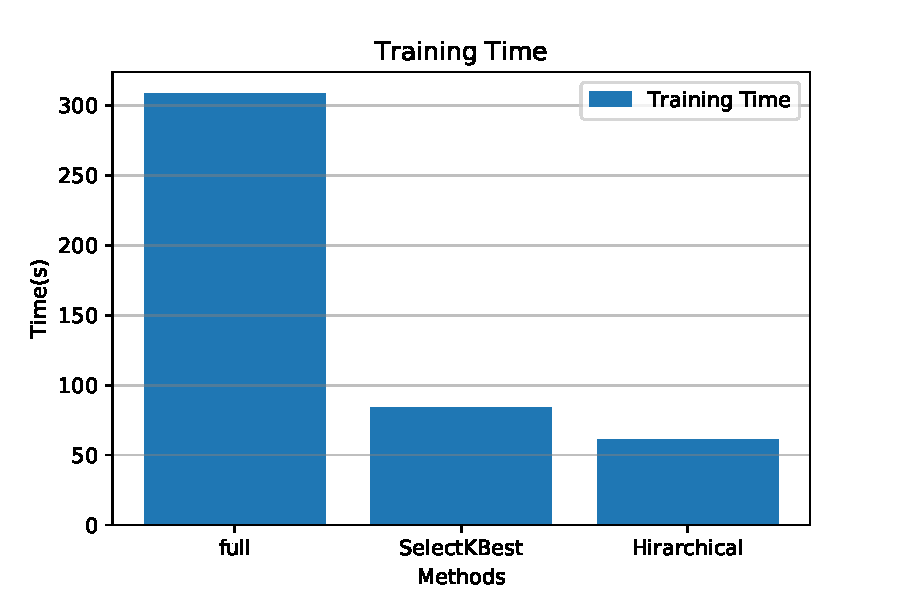
\includegraphics[scale=0.5]{fig/Training-Time.pdf}
    \caption{Training Time}
    \label{fig:training-time}
\end{figure}

\subsubsection{Metrics}

The metrics of model include accuracy, precision, recall and f1-score. The test result is shown in Table \ref{tab:metrics} and Figure \ref{fig:metrics}. The result indicates that Except that it is only slightly lower in accuracy, our model is generally better than the model trained with the full feature set. Besides, the model using the features selected by our method performs better than the model trained with the features selected by chi-square method.

\begin{table}[!htpb]
    \caption{Metrics Comparison}
    \label{tab:metrics}
    \centering
    \begin{tabular}{lrrr}
    \toprule
        & Hierarchical & Full & Chi-square \\
    \midrule
    Accuracy(\%) & \textbf{97.96} & 97.91 & 94.30 \\
    Precision(\%) & \textbf{80.40} & 81.38 & 72.43 \\
    Recall(\%) & \textbf{79.08} & 77.35 & 67.76 \\
    F1-Score(\%) & \textbf{79.14} & 78.52 & 68.78 \\
    \bottomrule
    \end{tabular}
\end{table}

\begin{figure}[!htbp]
    \centering
    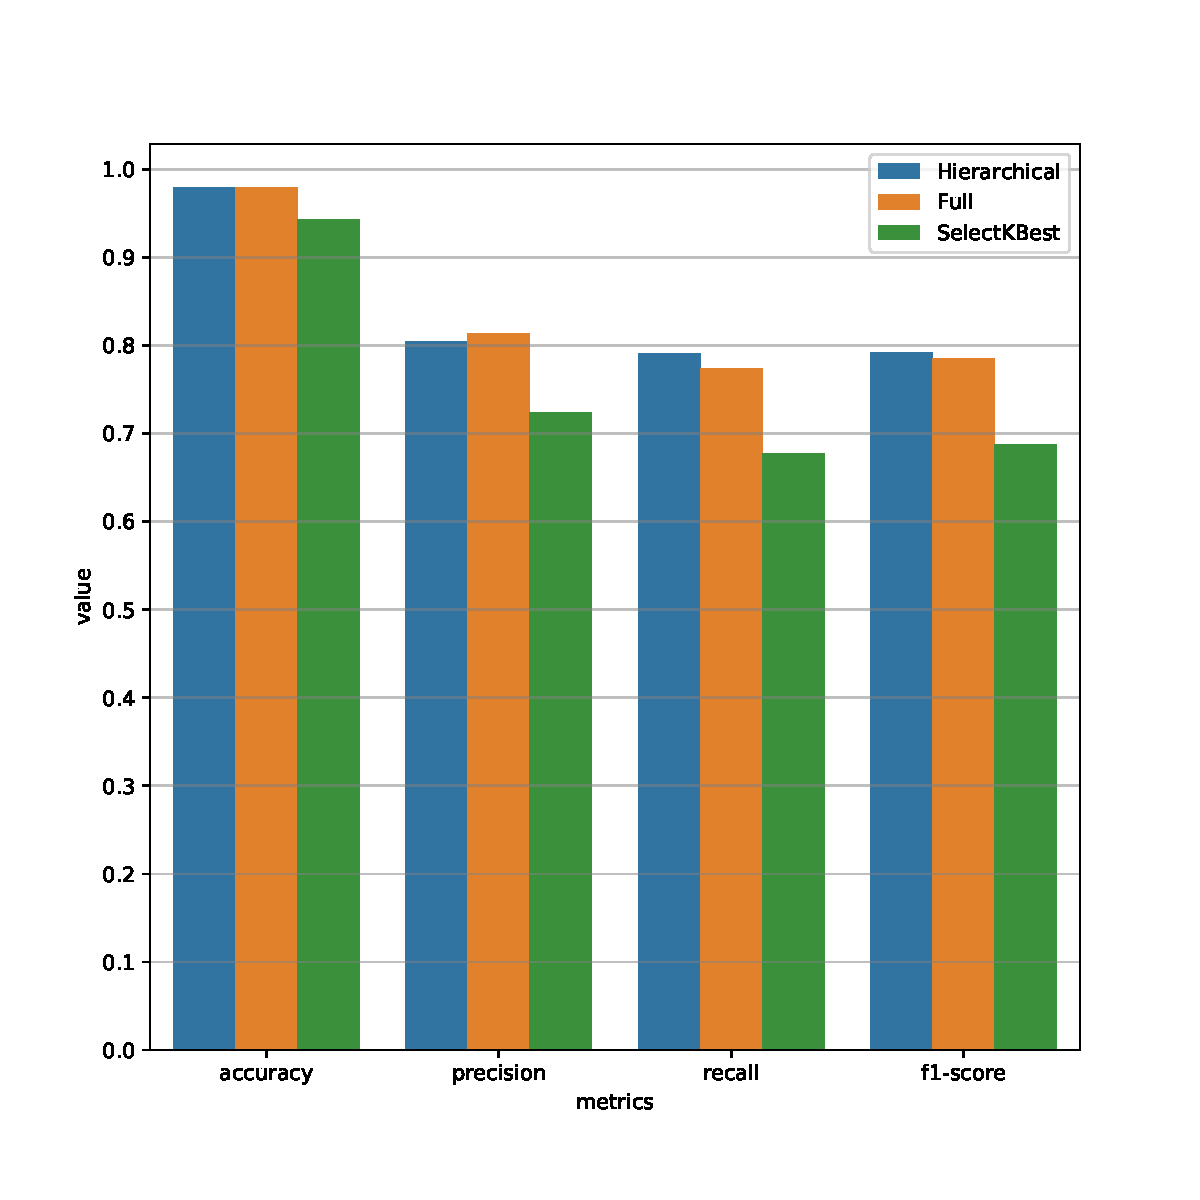
\includegraphics[scale=0.4]{fig/metrics.pdf}
    \caption{Accuracy, Precision, Recall and F1-score}
    \label{fig:metrics}
\end{figure}

\begin{figure*}[!htbp]
    \centering
    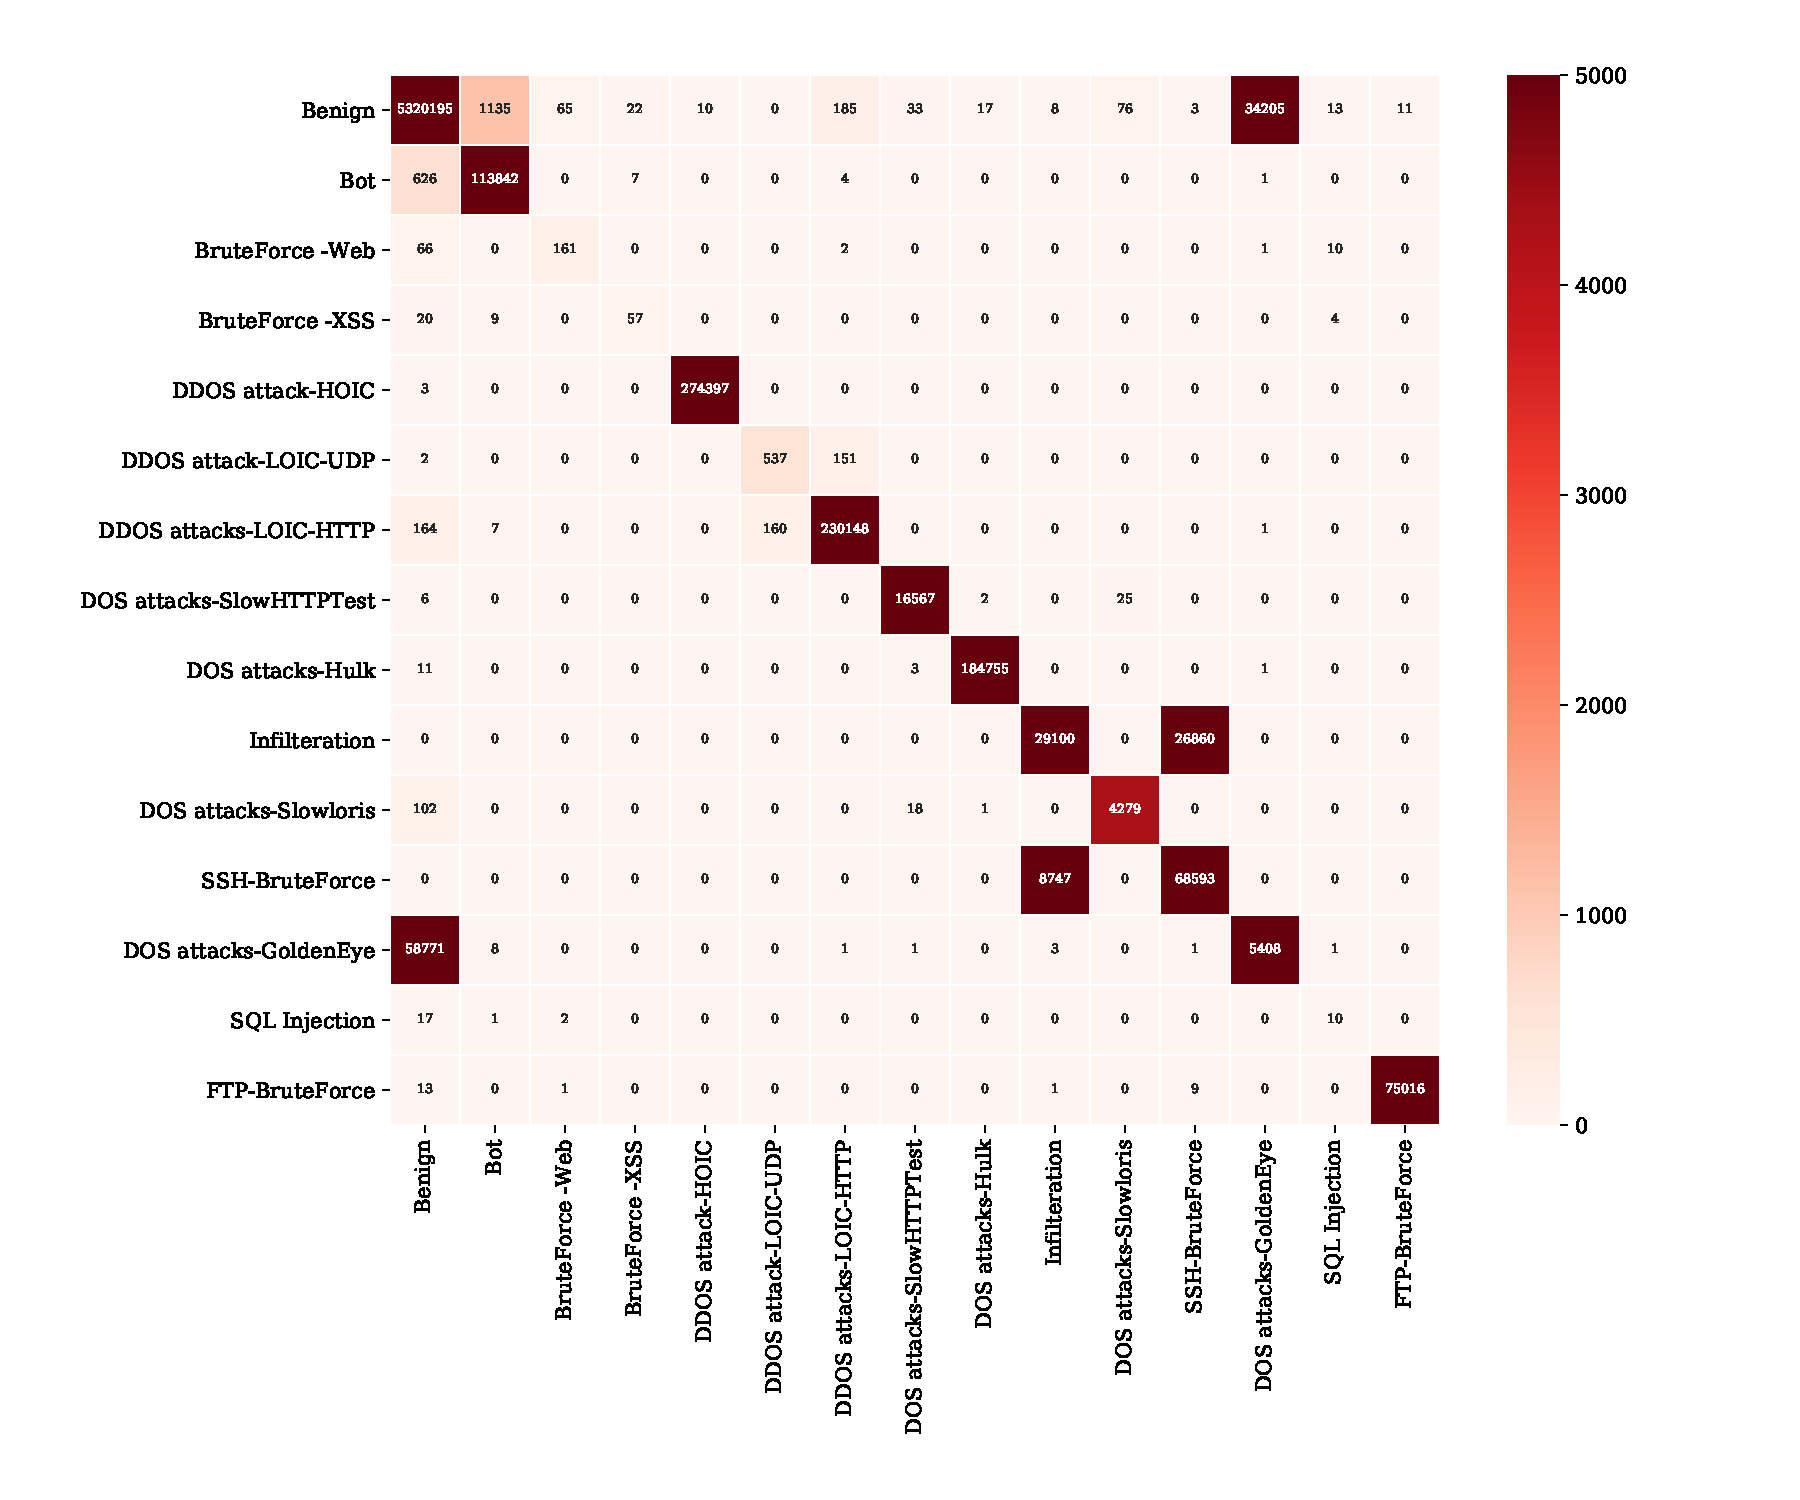
\includegraphics[scale=0.5]{fig/confusion-matrix.pdf}
    \caption{Heatmap of confusion matrix}
    \label{fig:confusion-matrix}
\end{figure*}

\subsection{Confusion Matrix}

\section{Discussion}
\label{sec:discussion}

\section{Conclusion}
\label{sec:conclusion}

This paper proposed a novel hierarchical feature selection method for network anomaly detection. We applied feature clustering algorithm using correlation-coefficient-based distance between features on network flow traffic data set, then ranked these feature cluster centers using information gain and information gain ratio simultaneously. After that we chose decision tree as our training algorithm to train the model based on the selected feature set. The experiment results shows our method can select more critical features which can determine whether a network flow is an attack. 

In the future, we will continue researching the methods of real-time network data analysis and real-time model of training and detection for network traffic.
% An example of a floating figure using the graphicx package.
% Note that \label must occur AFTER (or within) \caption.
% For figures, \caption should occur after the \includegraphics.
% Note that IEEEtran v1.7 and later has special internal code that
% is designed to preserve the operation of \label within \caption
% even when the captionsoff option is in effect. However, because
% of issues like this, it may be the safest practice to put all your
% \label just after \caption rather than within \caption{}.
%
% Reminder: the "draftcls" or "draftclsnofoot", not "draft", class
% option should be used if it is desired that the figures are to be
% displayed while in draft mode.
%
%\begin{figure}[!t]
%\centering
%\includegraphics[width=2.5in]{myfigure}
% where an .eps filename suffix will be assumed under latex, 
% and a .pdf suffix will be assumed for pdflatex; or what has been declared
% via \DeclareGraphicsExtensions.
%\caption{Simulation results for the network.}
%\label{fig_sim}
%\end{figure}

% Note that the IEEE typically puts floats only at the top, even when this
% results in a large percentage of a column being occupied by floats.


% An example of a double column floating figure using two subfigures.
% (The subfig.sty package must be loaded for this to work.)
% The subfigure \label commands are set within each subfloat command,
% and the \label for the overall figure must come after \caption.
% \hfil is used as a separator to get equal spacing.
% Watch out that the combined width of all the subfigures on a 
% line do not exceed the text width or a line break will occur.
%
%\begin{figure*}[!t]
%\centering
%\subfloat[Case I]{\includegraphics[width=2.5in]{box}%
%\label{fig_first_case}}
%\hfil
%\subfloat[Case II]{\includegraphics[width=2.5in]{box}%
%\label{fig_second_case}}
%\caption{Simulation results for the network.}
%\label{fig_sim}
%\end{figure*}
%
% Note that often IEEE papers with subfigures do not employ subfigure
% captions (using the optional argument to \subfloat[]), but instead will
% reference/describe all of them (a), (b), etc., within the main caption.
% Be aware that for subfig.sty to generate the (a), (b), etc., subfigure
% labels, the optional argument to \subfloat must be present. If a
% subcaption is not desired, just leave its contents blank,
% e.g., \subfloat[].


% An example of a floating table. Note that, for IEEE style tables, the
% \caption command should come BEFORE the table and, given that table
% captions serve much like titles, are usually capitalized except for words
% such as a, an, and, as, at, but, by, for, in, nor, of, on, or, the, to
% and up, which are usually not capitalized unless they are the first or
% last word of the caption. Table text will default to \footnotesize as
% the IEEE normally uses this smaller font for tables.
% The \label must come after \caption as always.
%
%\begin{table}[!t]
%% increase table row spacing, adjust to taste
%\renewcommand{\arraystretch}{1.3}
% if using array.sty, it might be a good idea to tweak the value of
% \extrarowheight as needed to properly center the text within the cells
%\caption{An Example of a Table}
%\label{table_example}
%\centering
%% Some packages, such as MDW tools, offer better commands for making tables
%% than the plain LaTeX2e tabular which is used here.
%\begin{tabular}{|c||c|}
%\hline
%One & Two\\
%\hline
%Three & Four\\
%\hline
%\end{tabular}
%\end{table}


% Note that the IEEE does not put floats in the very first column
% - or typically anywhere on the first page for that matter. Also,
% in-text middle ("here") positioning is typically not used, but it
% is allowed and encouraged for Computer Society conferences (but
% not Computer Society journals). Most IEEE journals/conferences use
% top floats exclusively. 
% Note that, LaTeX2e, unlike IEEE journals/conferences, places
% footnotes above bottom floats. This can be corrected via the
% \fnbelowfloat command of the stfloats package.

% if have a single appendix:
%\appendix[Proof of the Zonklar Equations]
% or
%\appendix  % for no appendix heading
% do not use \section anymore after \appendix, only \section*
% is possibly needed

% use appendices with more than one appendix
% then use \section to start each appendix
% you must declare a \section before using any
% \subsection or using \label (\appendices by itself
% starts a section numbered zero.)
%



% Can use something like this to put references on a page
% by themselves when using endfloat and the captionsoff option.
\ifCLASSOPTIONcaptionsoff
  \newpage
\fi



% trigger a \newpage just before the given reference
% number - used to balance the columns on the last page
% adjust value as needed - may need to be readjusted if
% the document is modified later
%\IEEEtriggeratref{8}
% The "triggered" command can be changed if desired:
%\IEEEtriggercmd{\enlargethispage{-5in}}

% references section

% can use a bibliography generated by BibTeX as a .bbl file
% BibTeX documentation can be easily obtained at:
% http://mirror.ctan.org/biblio/bibtex/contrib/doc/
% The IEEEtran BibTeX style support page is at:
% http://www.michaelshell.org/tex/ieeetran/bibtex/
\bibliographystyle{IEEEtran}
% argument is your BibTeX string definitions and bibliography database(s)
\bibliography{bibtex/bib/mybib.bib}
%
% <OR> manually copy in the resultant .bbl file
% set second argument of \begin to the number of references
% (used to reserve space for the reference number labels box)
%\begin{thebibliography}{1}

%\bibitem{IEEEhowto:kopka}
%H.~Kopka and P.~W. Daly, \emph{A Guide to \LaTeX}, 3rd~ed.\hskip 1em plus
%  0.5em minus 0.4em\relax Harlow, England: Addison-Wesley, 1999.

%\end{thebibliography}

% biography section
% 
% If you have an EPS/PDF photo (graphicx package needed) extra braces are
% needed around the contents of the optional argument to biography to prevent
% the LaTeX parser from getting confused when it sees the complicated
% \includegraphics command within an optional argument. (You could create
% your own custom macro containing the \includegraphics command to make things
% simpler here.)
%\begin{IEEEbiography}[{\includegraphics[width=1in,height=1.25in,clip,keepaspectratio]{mshell}}]{Michael Shell}
% or if you just want to reserve a space for a photo:

% \begin{IEEEbiography}{Michael Shell}
% Biography text here.
% \end{IEEEbiography}

% if you will not have a photo at all:
% \begin{IEEEbiographynophoto}{John Doe}
% Biography text here.
% \end{IEEEbiographynophoto}

% insert where needed to balance the two columns on the last page with
% biographies
%\newpage

% \begin{IEEEbiographynophoto}{Jane Doe}
% Biography text here.
% \end{IEEEbiographynophoto}

% You can push biographies down or up by placing
% a \vfill before or after them. The appropriate
% use of \vfill depends on what kind of text is
% on the last page and whether or not the columns
% are being equalized.

%\vfill

% Can be used to pull up biographies so that the bottom of the last one
% is flush with the other column.
%\enlargethispage{-5in}



% that's all folks
\end{document}


